\documentclass[10pt]{beamer}

\usetheme[progressbar=frametitle]{metropolis}
\usepackage{appendixnumberbeamer}

\usepackage[utf8]{inputenc}

\usepackage{booktabs}
\usepackage[scale=2]{ccicons}

\usepackage{pgfplots}
\usepgfplotslibrary{dateplot}

\usepackage{xspace}
\newcommand{\themename}{\textbf{\textsc{metropolis}}\xspace}

\title{Almacenamiento en la nube}
\subtitle{Dropbox}
% \date{\today}
\date{}
\author{Laura Sánchez Parra\\ Antonio Gámiz Delgado \\ Samuel Medina Gutiérrez }

\institute{Universidad de Granada.}
\titlegraphic{\hfill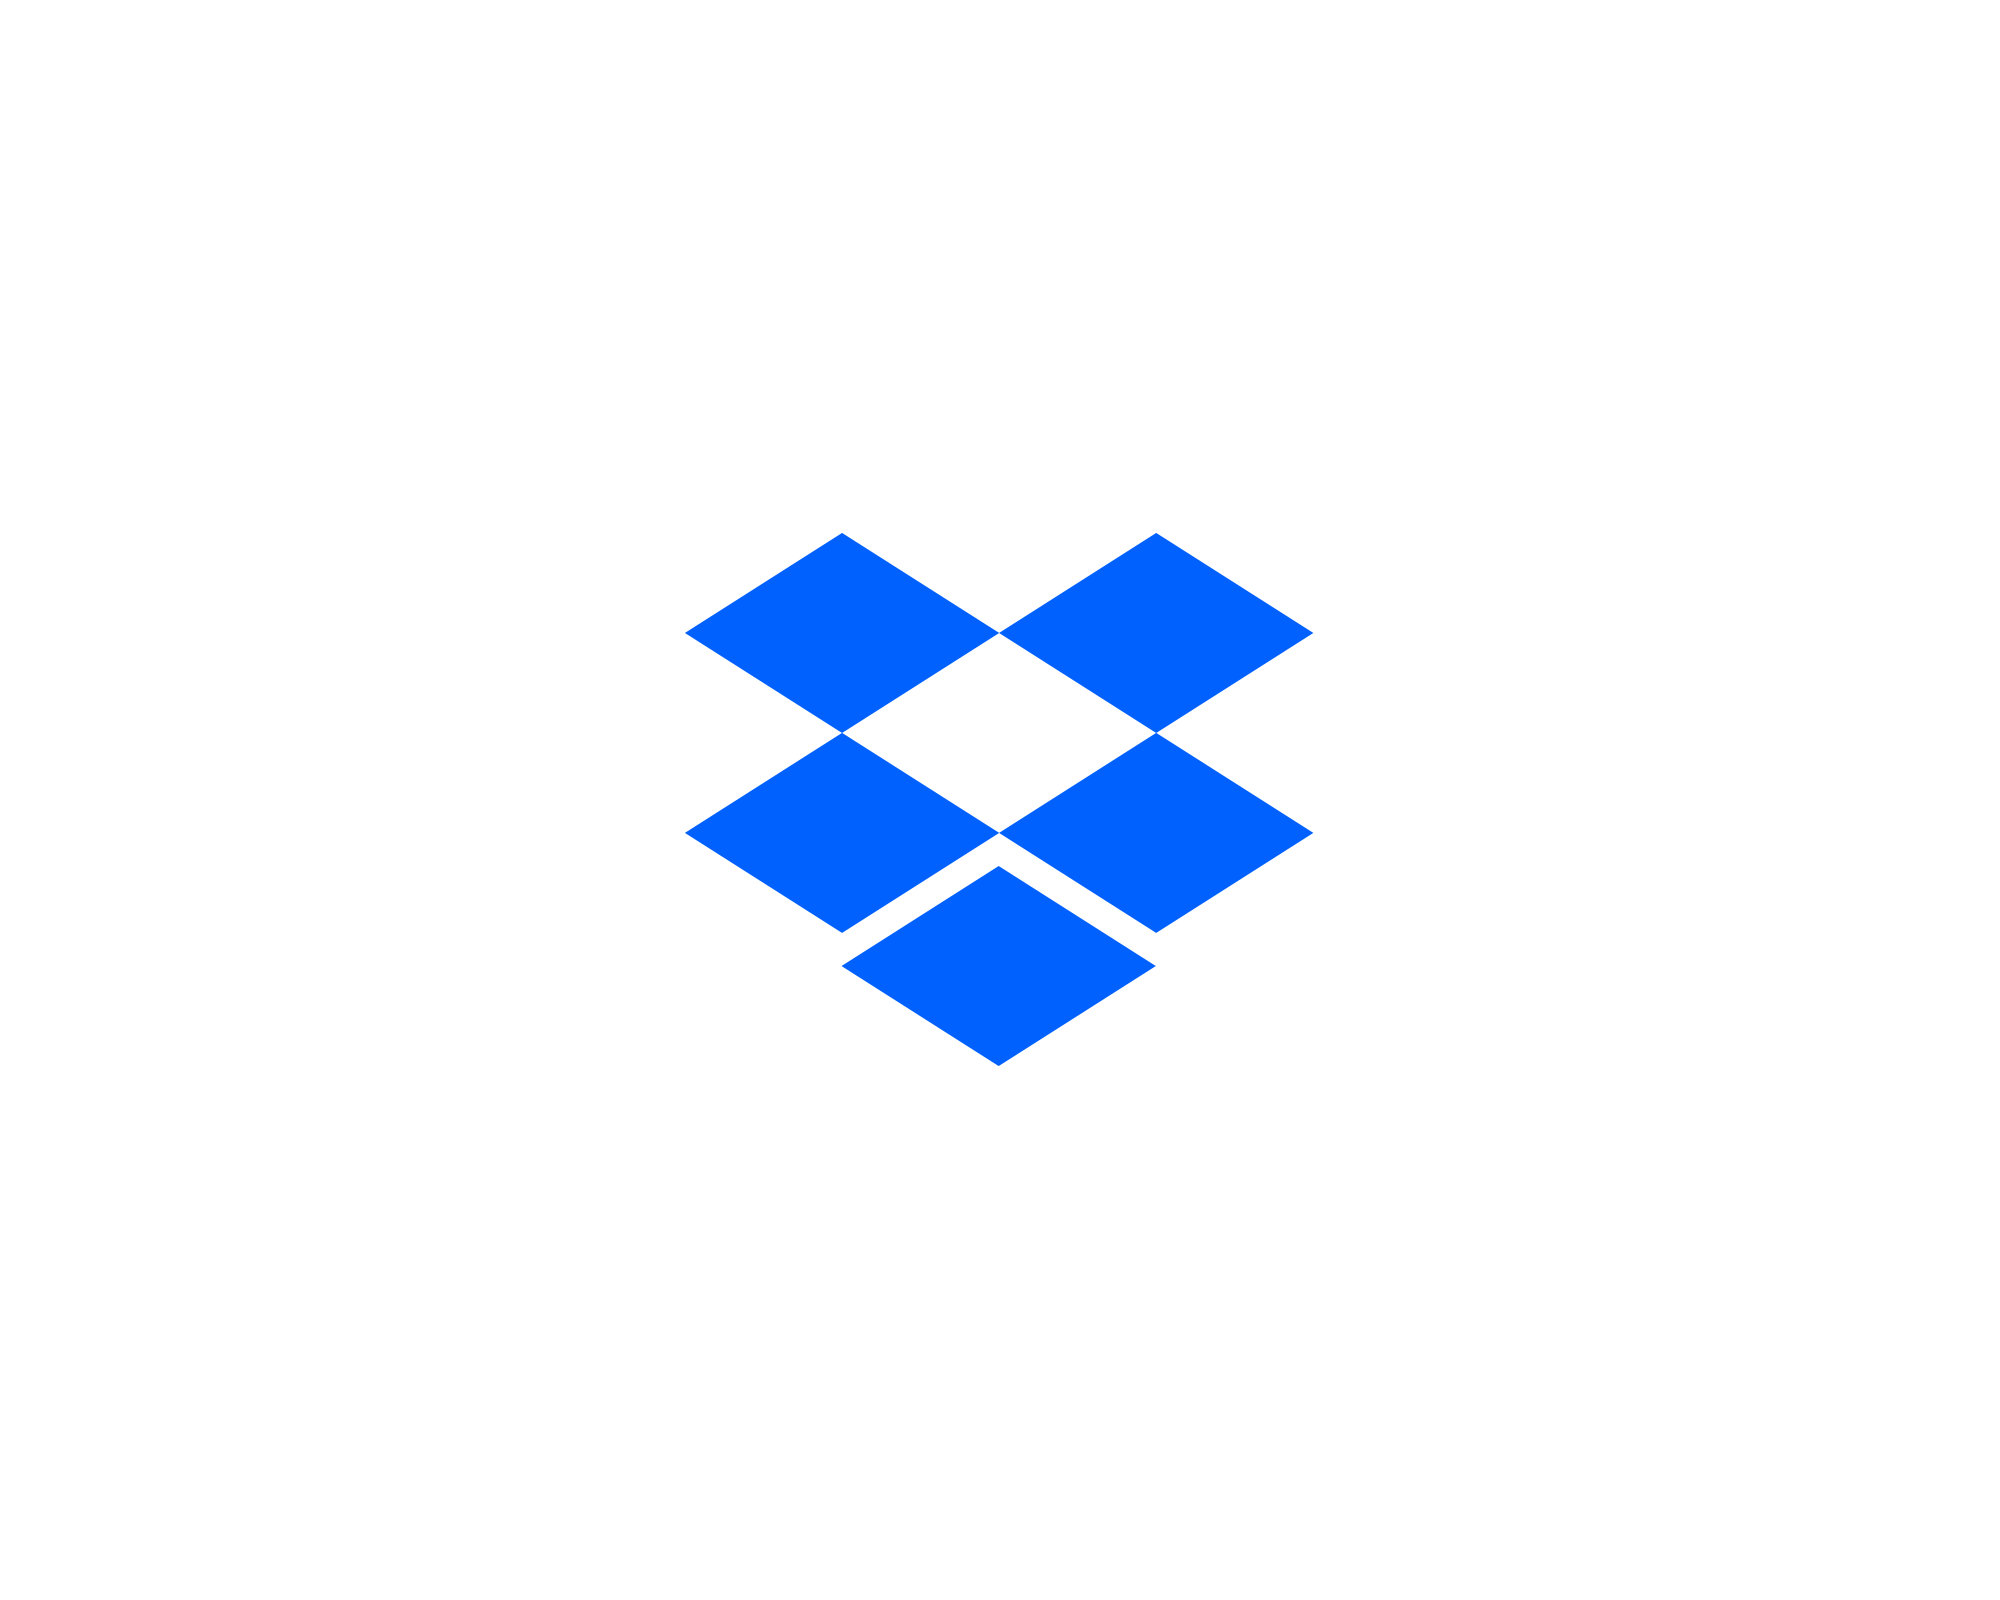
\includegraphics[height=4.5cm]{logo.png}}

\begin{document}

\maketitle

\begin{frame}{Índice}
  \setbeamertemplate{section in toc}[sections numbered]
  \tableofcontents[hideallsubsections]
\end{frame}

\section{Introducción}

\begin{frame}[fragile]{Cloud-Storage}
\begin{alertblock}{Definición}
Cloud-Storage es un modelo de servicio en el cual los datos son mantenidos, distribuidos, administrados y puestos a la disposición de los usuarios en una red (normalmente Internet).
\end{alertblock}
\begin{alertblock}{Ventajas}
\begin{itemize}
\item Facilidad de acceso a los archivos
\item Multiplataforma
\item Facilidad de recuperación de datos
\item Ahorro de costes
\end{itemize}
\end{alertblock}

\end{frame}

\section{Sistemas de almacenamiento}

\begin{frame}{Principales sistemas de almacenamiento}
\begin{alertblock}{Definición}
Un sistema de almacenamiento consiste en habilitar uno o varios discos duros de una red local (que a su vez puede estar conectada a Internet) de manera que los datos almacenados sean accesibles a todos los dispositivos que deseen utilizarlos.
\end{alertblock}
\begin{alertblock}{Tipos}
\begin{itemize}
\item Network Attached Storage (NAS)
\item Storage Area Network (SAN)
\item Direct Access Storage (DAS)
\end{itemize}
\end{alertblock}
\end{frame}

\subsection{Network Attached Storage - NAS}

\begin{frame}{Network Attached Storage - NAS}
\begin{alertblock}{NAS}
Este sistema incorpora su propio sistema de conexión y recepción de petición de acceso a los datos, eliminando a los servidores de la ecuación. Los sitemas de almacenamiento NAS se conectan directamente al router (LAN) y usan TCP/IP cómo protocolo.
\end{alertblock}
\end{frame}

\begin{frame}{Network Attached Storage - NAS}
\begin{figure}[h]
\center
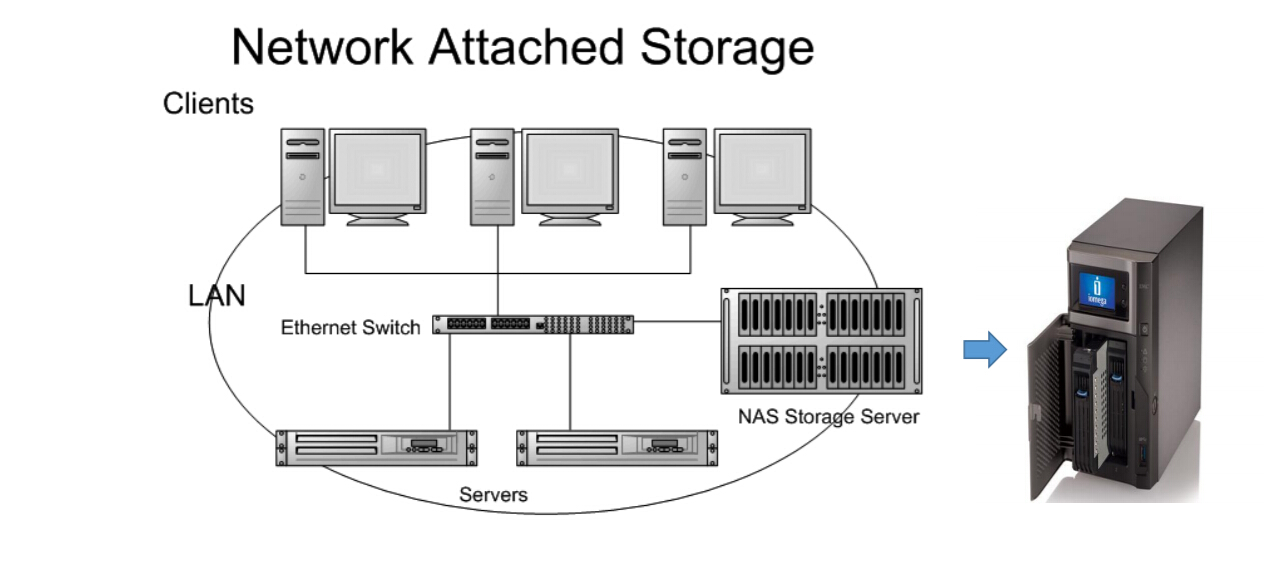
\includegraphics[scale=0.35]{nas.jpg}
\end{figure}
\end{frame}

\begin{frame}{Network Attached Storage - NAS}
\begin{alertblock}{Ventajas}
\begin{itemize}
\item Todos los usuarios conectados a la misma red que el NAS, pueden acceder a él.

\item Seguro, ya que somos nosotros mismos quienes manipulamos los archivos.
\end{itemize}
\begin{alertblock}{Incovenientes}
\begin{itemize}
\item Difícil instalación correcta.
\item Un poco caro.
\end{itemize}
\end{alertblock}

\end{alertblock}

\end{frame}

\subsection{Storage Area Network - SAN}

\begin{frame}{Storage Area Network - SAN}
\begin{alertblock}{SAN}
Como un NAS, SAN traspasa la responsabilidad de almacenar datos de los servidores a dispositivos de almacenamiento dedicados. Pero a diferencia del NAS, un SAN es una red de dispositivos de almacenamiento interconectados, accedidos a través de la red local.
\end{alertblock}
\end{frame}

\begin{frame}{Storage Area Network - SAN}
\begin{figure}[h]
\center
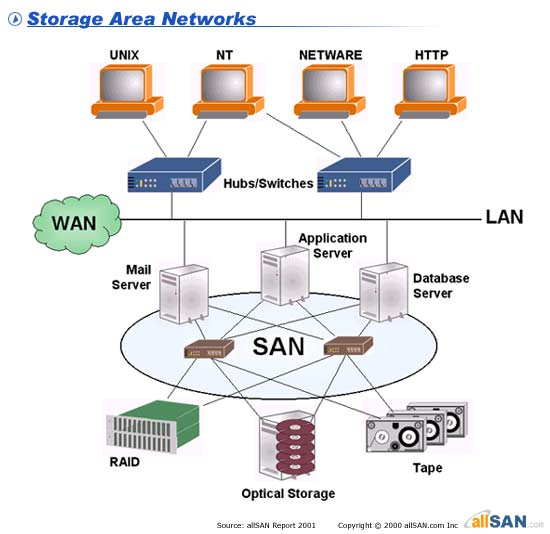
\includegraphics[scale=0.4]{san.jpg}
\end{figure}
\end{frame}

\begin{frame}{Storage Area Network - SAN}
\begin{alertblock}{Ventajas}
\begin{itemize}
\item Expansión de capacidad de almacenamiento prácticamente ilimitado.
\item Tráfico del SAN (fibra) totalmente separado del tráfico de usuario (ethernet).
\end{itemize}
\begin{alertblock}{Incovenientes}
\begin{itemize}
\item Rendimiento muy dependiente del tipo de red usado.
\item Más cara que el NAS.
\end{itemize}
\end{alertblock}

\end{alertblock}

\end{frame}

\subsection{Direct Access Storage - DAS}

\begin{frame}{Direct Access Storage - DAS}
\begin{alertblock}{DAS}
Son todos los dispositivos USB, discos duros, CDs, etc, que se conectan con un computador y se tiene acceso directo al almacenamiento.
\end{alertblock}

\begin{figure}[h]
\center
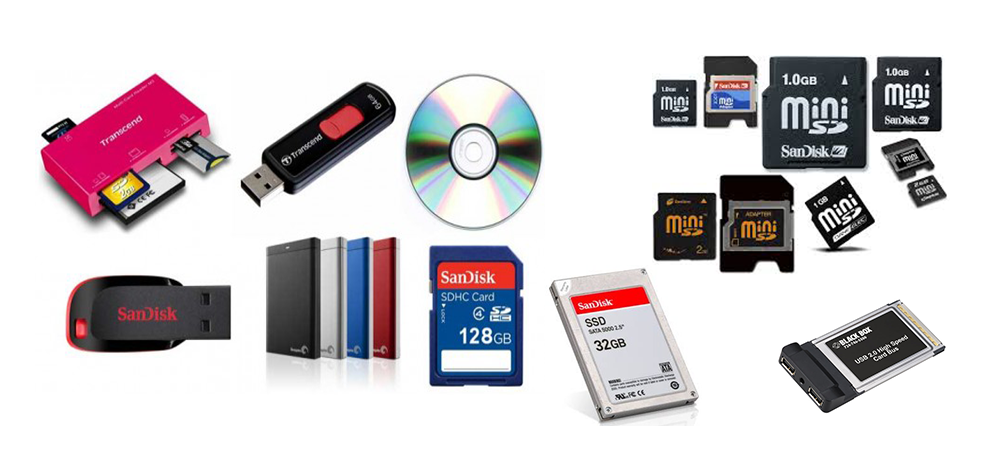
\includegraphics[scale=4]{das.png}
\end{figure}
\end{frame}

\section{Protocolos de almacenamiento}

\subsection{Small Computer System Interface - SCSI}

\begin{frame}{Small Computer System Interface - SCSI}
\begin{alertblock}{SCSI}
Es el principal método de acceso a disco en el centro de datos. El
acceso a disco es realizado por medio de bloque. Este protocolo permite al servidor acceder directamente a los bloques del disco sin necesidad de un sistema de archivos.
\end{alertblock}
\begin{figure}[h]
\center
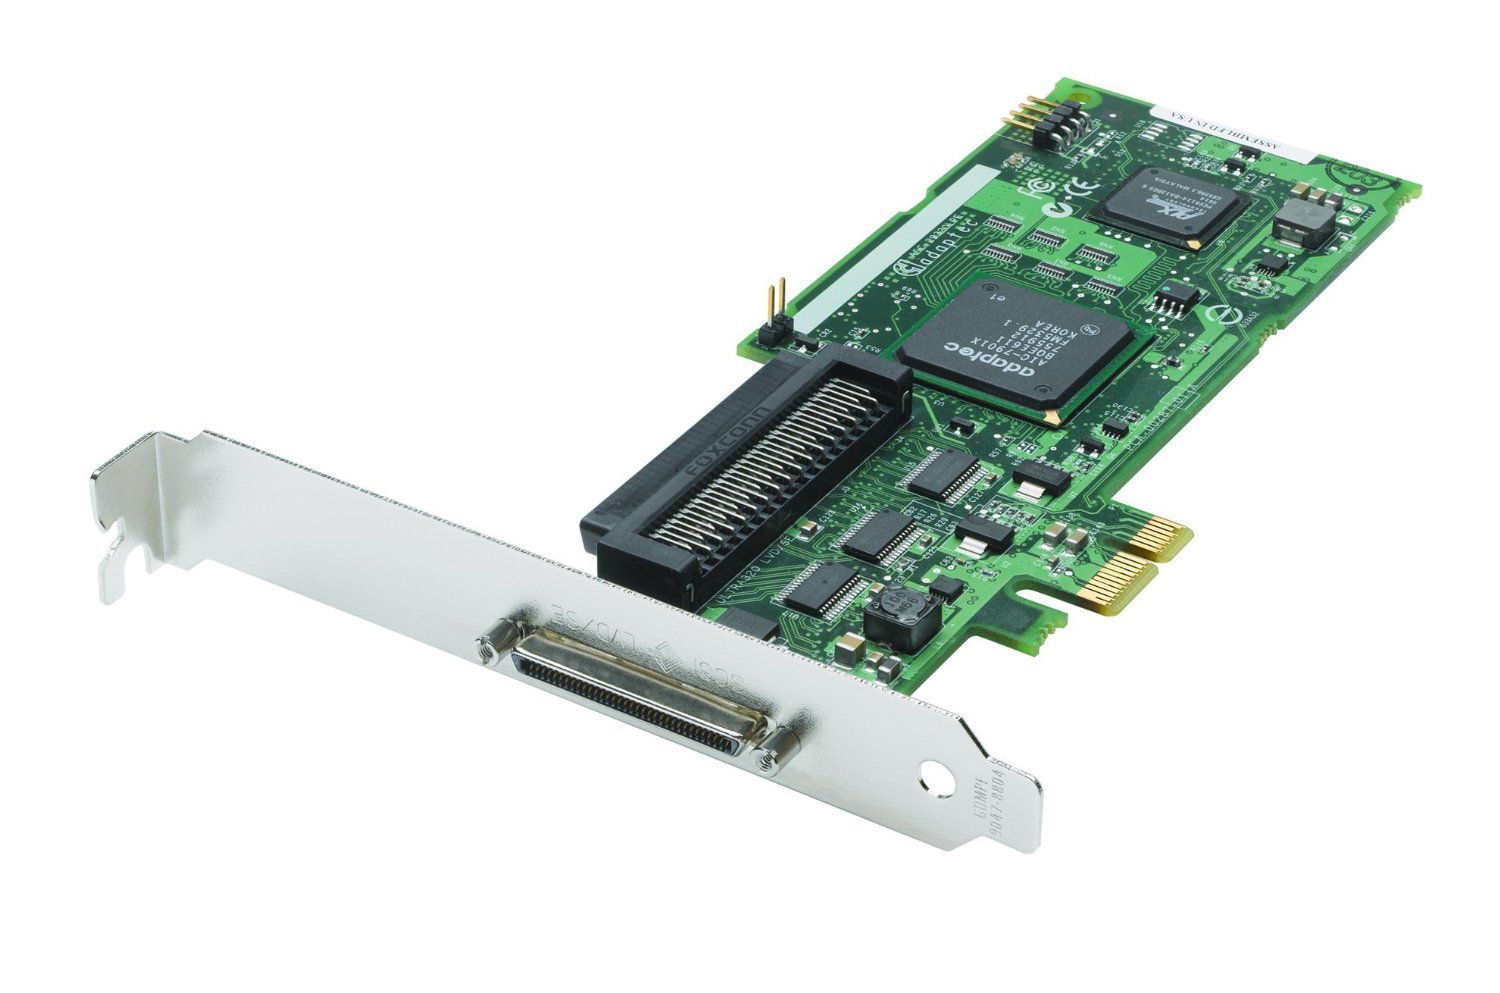
\includegraphics[scale=0.13]{scsi.jpg}
\end{figure}

\end{frame}
\begin{frame}{Small Computer System Interface - SCSI}
\begin{figure}[h]
\center
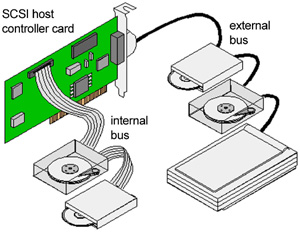
\includegraphics[scale=0.9]{scsi1.jpg}
\end{figure}
\end{frame}

\subsection{Fiber Channel - FC}

\begin{frame}{Fiber Channel - FC}
\begin{alertblock}{FC}
Encapsula datos del protocolo SCSI y Command Descriptor Blocks
(CDB) en ”cargas de trabajo” del canal de fibra. Una vez encapsulados, las
red FC se encarga del direccionamiento, enrutamiento y del control de flujo
requerido para soportar SCSI.
\end{alertblock}
\begin{figure}[h]
\center
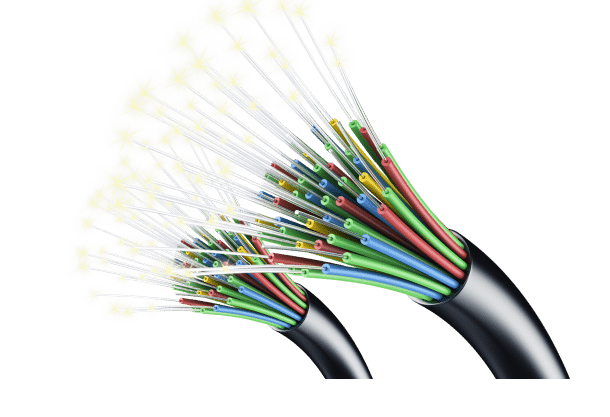
\includegraphics[scale=0.35]{fc.png}
\end{figure}

\end{frame}
\begin{frame}{Fiber Channel - FC}
\begin{figure}[h]
\center
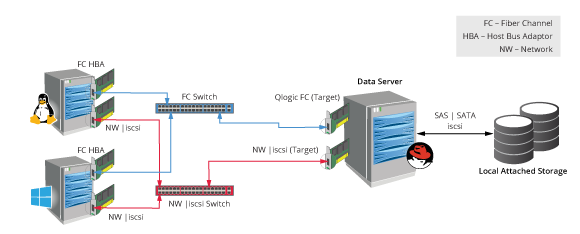
\includegraphics[scale=0.58]{fc1.png}
\end{figure}
\end{frame}

\subsection{internet/IP Small Computer System Interface - iSCSI}

\begin{frame}{internet/IP Small Computer System Interface - iSCSI}
\begin{alertblock}{iSCSI}
Coge los datos del SCSI y los CDM y los encapsula en paquetes TCP/IP, al que igual que FC.
\end{alertblock}
\begin{alertblock}{Ventajas}
La principal atracción de iSCSI es que el almacenamiento de datos puede ser fácilmente extendido entre la infraestructura existente con un coste adicional mínimo.
\end{alertblock}

\begin{alertblock}{Incovenientes}
\begin{itemize}
\item Antiguos cables Ethernet de 1GE.
\item Encapsula al protocolo SCSI.
\end{itemize}
\end{alertblock}
\end{frame}
\begin{frame}{internet/IP Small Computer System Interface - iSCSI}
\begin{figure}[h]
\center
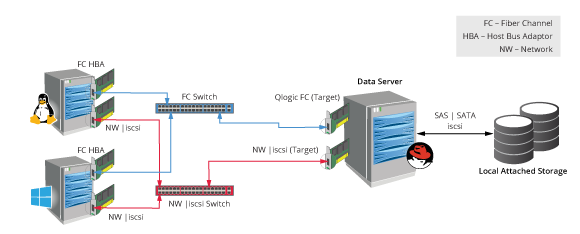
\includegraphics[scale=0.58]{fc1.png}
\end{figure}
\end{frame}


\subsection{Fiber Channel over Ethernet - FCoE}

\begin{frame}{Fiber Channel over Ethernet - FCoE}
\begin{alertblock}{FCoE}
Protocolo que se encarga de proveer la funcionalidad necesaria para ejecutar el protocolo FC sobre una red Ethernet (10GE). FCoE encapsula los paquetes del protocolo FC en paquetes Ethernet Jumbo, que aseguran que el paquete no es ni fragmentado ni alterado.
\end{alertblock}
\begin{alertblock}{Ventajas}
Permite integrar la red Ethernet y el canal de fibra en uno solo, facilitanto los diseños.
\end{alertblock}
\end{frame}

\begin{frame}{Fiber Channel over Ethernet -  FCoE}
\begin{figure}
\centering
\begin{minipage}{.5\textwidth}
  \centering
  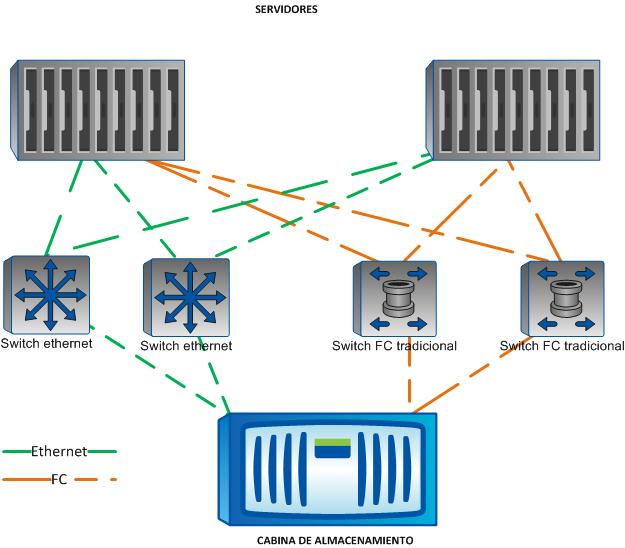
\includegraphics[width=.8\linewidth]{fcoe1.jpg}
  \caption{FC+E}
\end{minipage}%
\begin{minipage}{.5\textwidth}
  \centering
  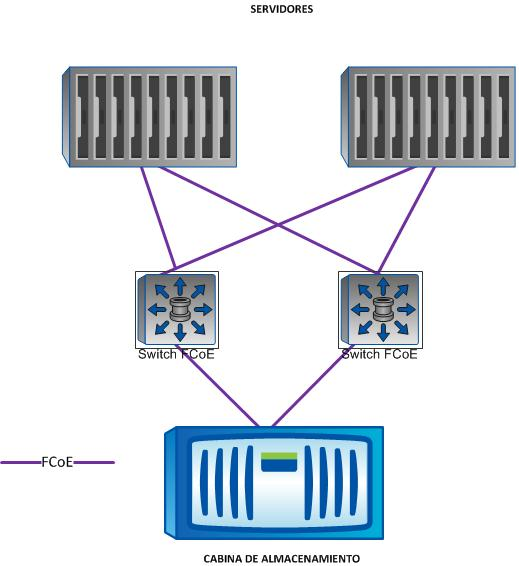
\includegraphics[width=.8\linewidth]{fcoe2.jpg}
  \caption{FCoE}
\end{minipage}
\end{figure}
\end{frame}

\subsection{Y muchos más...}

\begin{frame}{Y muchos más...}
\begin{alertblock}{Common Internet File System - CIFS}
Normalmente usado por Microsoft para compartir archivos.
\end{alertblock}
\begin{alertblock}{Network File System - NFC}
Usado en entornos Unix/Linux y en máquinas virtuales.
\end{alertblock}
\begin{alertblock}{Hyper Text Transfer Protocol - HTTP}

Los protocolos listados anteriormente normalmente se usan en los centros de datos, por lo que cuando nos traladamos al nivel de los proveedores (Google, etc), sufren un gran problema de escalabilidad. Ahí es donde entre el protocolo HTTP para simplificar la configuración del almacenaje e incrementar su escalabilidad.

\end{alertblock}
\end{frame}

\begin{frame}{Y muchos más...}
\begin{alertblock}{¿Y cómo o cuáles usa Dropbox?}
\end{alertblock}
\end{frame}


\section{Dropbox}

\begin{frame}{Dropbox}
\begin{alertblock}{Historia}
Dropbox es un servicio de almacenamiento en la nube, creado por Drew Houston y Arash Ferdowsi en junio de 2007.
\end{alertblock}
\begin{figure}[h]
  \centering
  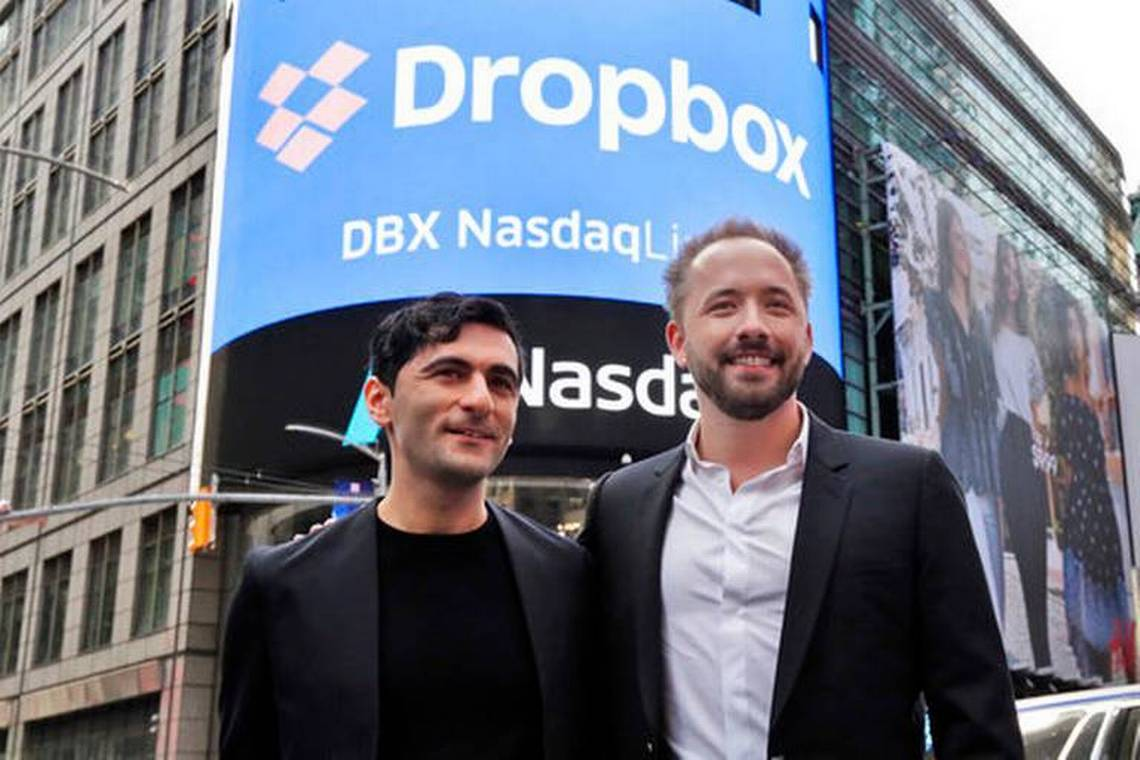
\includegraphics[width=0.7\linewidth]{fundadores.jpg}
  \caption{Fundadores}
\end{figure}
\end{frame}

\begin{frame}{Dropbox}
\begin{alertblock}{¿Qué es Dropbox?}
Dropbox se define a si mismo como una CDN (Content Delivery Network). Usan los protocolos TCP/IP y TLS para el manejo de la información, ya que reducen la latencia.
\end{alertblock}
\begin{figure}[h]
  \centering
  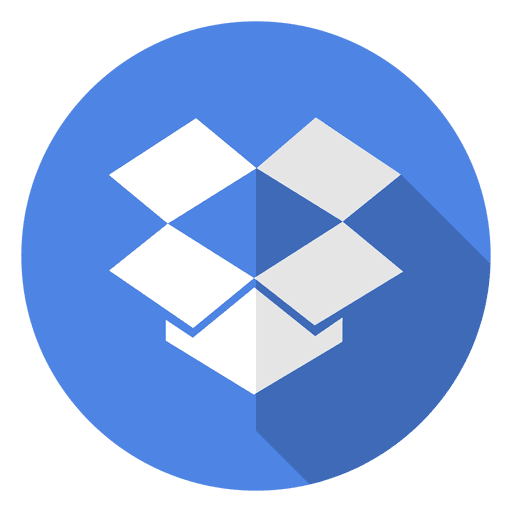
\includegraphics[width=0.4\linewidth]{logo2}
\end{figure}
\end{frame}

\begin{frame}{Edge Network}
\begin{figure}[h]
  \centering
  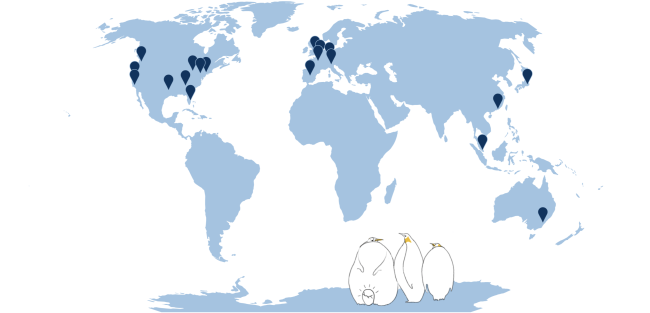
\includegraphics[width=1\linewidth]{pop}
  \caption{PoPs actuales}
\end{figure}

\end{frame}

\begin{frame}{Edge Network}
\begin{figure}[h]
  \centering
  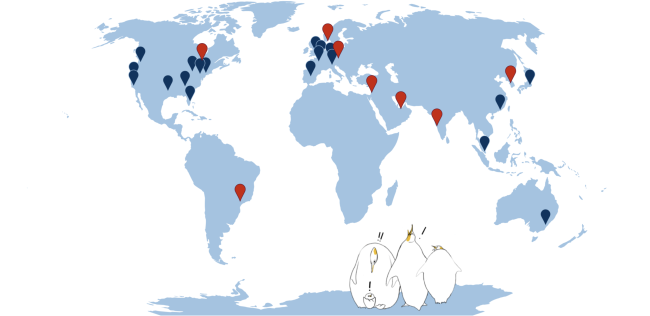
\includegraphics[width=1\linewidth]{pop2}
  \caption{PoPs esperadaos para 2019}
\end{figure}

\end{frame}

\begin{frame}{Edge Network}
\alert{¿Por qué es importante la Edge Network?}
\begin{figure}[h]
  \centering
  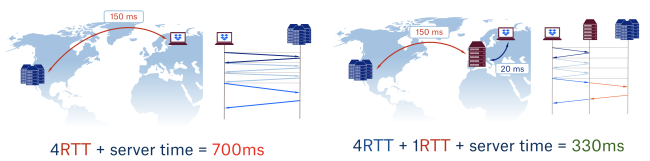
\includegraphics[width=1\linewidth]{pop3}
\end{figure}

\end{frame}
\begin{frame}{Edge Network}
\alert{¿Por qué es importante la Edge Network?}
\begin{figure}[h]
  \centering
  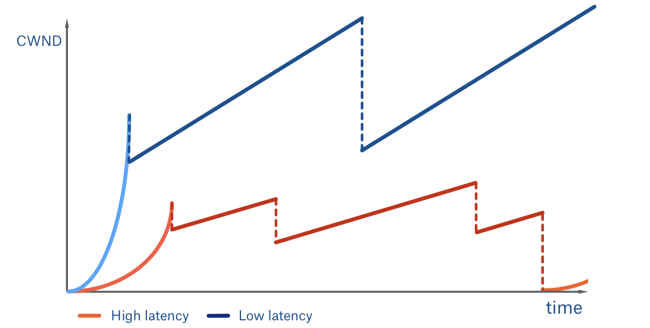
\includegraphics[width=1\linewidth]{pop4}
\end{figure}

\end{frame}

\begin{frame}{Global Server Load Balancer - GSLB}
\begin{alertblock}{¿Cómo distribuye Dropbox los usuarios entre los PoPs?}
Utiliza Global Server Load Balancer (GSLB), que consiste en enviar a cada usuario al PoP más cercano, a no ser que esté deshabilitado. Hay varias formas de repartir los usuarios.
\end{alertblock}

\end{frame}

\begin{frame}{Global Server Load Balancer - GSLB}
\begin{alertblock}{GBP Anycast}
Usa el protocolo de routing del núcleo de Internet, BGP (Border Gateway Protocol). Consiste en "publicar" la misma subred desde todos los PoPs, e Internet entregará cada paquete al PoP más óptimo.
\end{alertblock}
\begin{figure}[h]
  \centering
  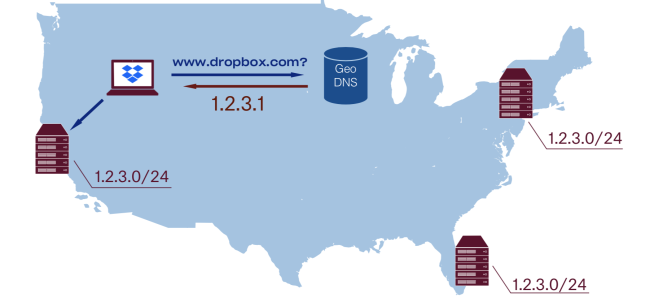
\includegraphics[width=1\linewidth]{gbp}
\end{figure}
\end{frame}


\begin{frame}{Global Server Load Balancer - GSLB}
\begin{alertblock}{GeoDNS}
Cada PoP tiene su propio y único espacio de direcciones IP y DNS es el responsable de asignar una IP diferente a cada usuario basado en su localización geográfica. Enrutamiento basado en LatLog (muy complejo).
\end{alertblock}
\begin{figure}[h]
  \centering
  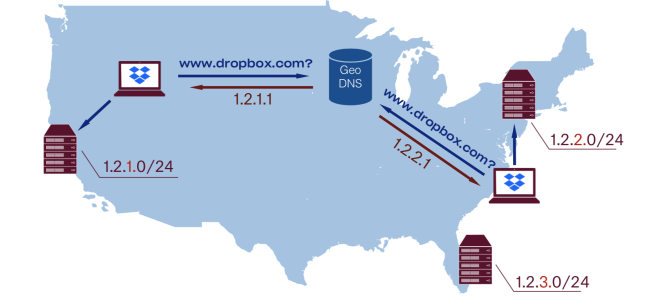
\includegraphics[width=1\linewidth]{geodns}
\end{figure}
\end{frame}

\begin{frame}{Global Server Load Balancer - GSLB}
\begin{alertblock}{Hybrid Unicast/Anycast}
Combinación de las dos anteriores, que permite beneficiarse de las ventajas de los dos métodos anteriores.
\end{alertblock}
\begin{figure}[h]
  \centering
  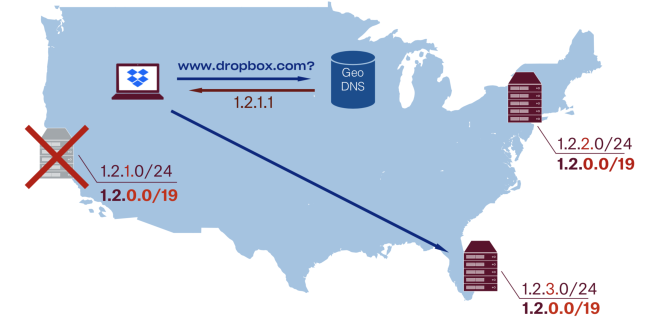
\includegraphics[width=1\linewidth]{hybrid}
\end{figure}
\end{frame}

\begin{frame}{Global Server Load Balancer - GSLB}
\begin{alertblock}{Real Users Metric (RUM)}
Combinación de las dos anteriores, que permite beneficiarse de las ventajas de los dos métodos anteriores.
\end{alertblock}
\begin{figure}[h]
  \centering
  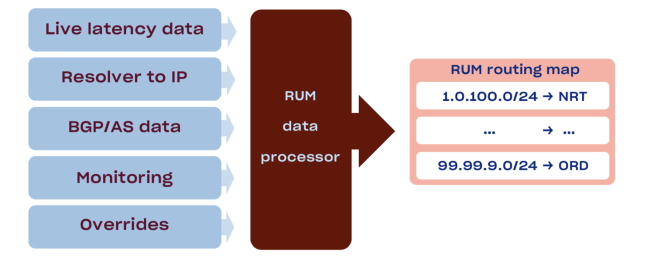
\includegraphics[width=1\linewidth]{rum}
\end{figure}
\end{frame}

\begin{frame}{Backbone Network}
\begin{alertblock}{¿Qué es?}
Red de interconexión entre los data centers y los PoPs. Consiste en gestionar interfaces en múltiples redes cuya tarea es copiar paquetes de una red a otra en función de las tablas de enrutamiento almacenadas en la memoria.
\end{alertblock}
\end{frame}

\begin{frame}{Backbone Network}
\begin{figure}[h]
  \centering
  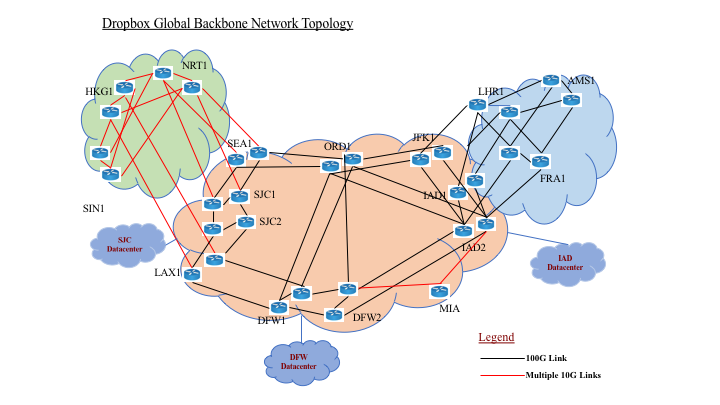
\includegraphics[width=1\linewidth]{backbone}
\end{figure}
\end{frame}

\begin{frame}{Backbone Network (internamente)}
\begin{alertblock}{Interior Gateway Protocol (IGP)}
Gestiona interfaces en múltiples redes cuya tarea es copiar paquetes de una red a otra en función de las tablas de enrutamiento almacenadas en memoria.
\end{alertblock}
\begin{alertblock}{Open Shortest Path First (OSPF)}
Usa el algoritmo de Dijkstra para calcular la ruta más corta entre dos nodos.
\end{alertblock}
Actualmente Dropbox utiliza IPv6.
\end{frame}

\begin{frame}{Backbone Network (externamente)}
\begin{alertblock}{Diseño BGP}
Malla completa de todos los routers en todos los routers, es decir, todos los routers conocen todas las rutas entre sí.
\end{alertblock}
\begin{alertblock}{División de la red troncal}
Consiste en dividir la red troncal en regiones más pequeñas, a la vez que se usa BGP de malla completa entre los routers de una misma región.
\end{alertblock}
\end{frame}

\begin{frame}{Backbone Network}
\begin{figure}[h]
  \centering
  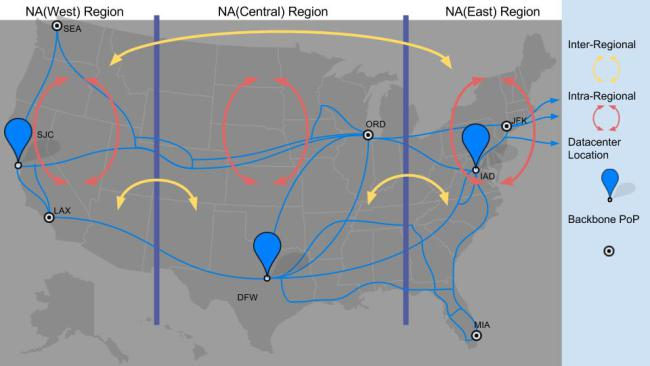
\includegraphics[width=1\linewidth]{bb2}
\caption{División de la red troncal}
\end{figure}
\end{frame}

\begin{frame}{Backbone Network}
\begin{alertblock}{¿Qué routers componen esta red?}
\begin{itemize}
\item Routers del centro de datos (DR): cuya función principal es conectrar el centro de datos a la red troncal.
\item Routers de red troncal (BB): actúan como un punto de terminación para circuitos de larga distancia y también como dispositivos de agregación para DR en regiones donde tenemos centros de datos.
\item Peering routers (PR): cuya función principal es conectar Dropbox a pares BGP externos para proporcionar conectividad a Internet.
\end{itemize}
\end{alertblock}
\end{frame}

\begin{frame}{Backbone Network}
\begin{figure}[h]
  \centering
  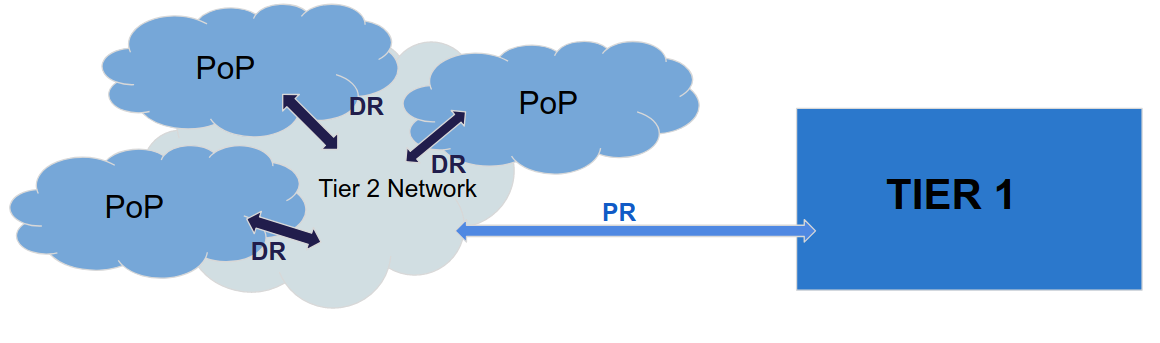
\includegraphics[width=1\linewidth]{bb3}
\end{figure}
\end{frame}


\section{Dropbox LAN Sync}

% Parte de Samuel

\begin{frame}{Fin}
\begin{figure}[h]
  \centering
  
\includegraphics[width=0.78\linewidth]{fin}
\end{figure}
\end{frame}

\end{document}

